\documentclass{article}
\usepackage[utf8]{inputenc}
\usepackage{listings}
\usepackage{minted}
\usepackage{biblatex}
\usepackage{hyperref}
\usepackage{amsmath}
\usepackage{graphicx}
\usepackage[left=3cm,right=3cm]{geometry}
\usepackage{caption}
\usepackage{titling}
\renewcommand\maketitlehooka{\null\mbox{}\vfill}
\renewcommand\maketitlehookd{\vfill\null}


\title{Report for Final Bomberman Project}
\author{Samuel Melm, Jonas Gann}
\date{March 2022}

\begin{document}
\begin{titlingpage}
\maketitle
\end{titlingpage}

\tableofcontents
\newpage

\section[Introduction]{Introduction {\small - Samuel Melm}}
% Introduction. State the problem you are trying to solve and give a brief overview of available methods

We want to train an agent to play the bomberman game. In this game, an agent can move over a 2D grid and place bombs. The agent that has the most points at the end wins. Points are gained by eliminating opponents and collecting coins, which are randomly hidden under boxes that need to be destroyed by bombs first. An agent has to look at the state of the board and select one of six actions (up, down, left, right, wait or bomb) to perform. We want the agent to choose actions which eventually result in the highest rewards. The problem can be restated as finding a function that expresses how optimal an action is, depending on the current board state. The following subsections introduce the most important machine learning methods and concepts used throughout this project.

\subsection[Reinforcement Learning]{Reinforcement Learning {\small - Samuel Melm}}
The goal of reinforcement learning is to teach an agent how to interact with an environment. The agent can carry out actions that act upon the environment. The agent can base these actions on observations it makes about the environment and on the reward it receives, which tells the agent how beneficial or detrimental they are towards its goal. 

By this description, it becomes quite obvious that the game of bomberman -- or nearly any game for that matter -- is a perfect scenario for reinforcement learning. There is an environment in the form of the playing field about which observations can be made (e.g., position of coins, bombs, and opponents) and the agent can perform actions (e.g., movement or placing a bomb). The goal of the agent is to achieve the highest possible score, which can function as a primitive reward function.

% What is reinforcement learning and why is it relevant for the project

\subsection[Q-Learning]{Q-Learning {\small - Samuel Melm}}

In any game there are good and bad situations as well as right or wrong decisions which depend on what situation the agent is in. Learning how to play a game well can therefore be boiled down to learning what action is good in which situation -- or state, as they are usually called. In games where the agent can determine the state an action would cause\footnote{like chess} it is enough for it to simply learn how good each state is. The rest can be archived by simply looking ahead to find the most desirable state. Bomberman is not such a game, since at any steps the behavior of the opponents cannot be deterministically predicted by the agent. Because of this, our agent needs to learn how good an action is depending on the current state. The simplest way to achieve this, is to keep a table where for each state action pair a value for the goodness of the pair is stored. This is called a Q-table. That approach does not perform well in a game like bomberman, since that table would be too big. By just considering the position of four agents \footnote{which can be on any of the 176 tiles} and their bombs \footnote{which can be on 20 reachable tiles around the agent or not placed at all} as the state, we would have a Q-table of size

\begin{align*}
    \mid Q \mid &= \# \textsf{agent positions} \cdot \# \textsf{bomb positions} \cdot \# \textsf{possible actions} \\
    &= {176 \choose 4} \cdot {21 \choose 4 } \cdot 7 \\
    &= 38630900 \cdot 5985 \cdot 7 \\
    &= 1.6184416 \cdot 10^{12}
\end{align*}

which does not include the position of crates, coins or explosions. A tabular approach to reinforcement learning does not work well with missing data. When a state action pair was not tried during training, the agent can only guess the value. Since this is not feasible, we need another approach.


\subsection[Regression]{Regression {\small - Samuel Melm}}

Since we cannot store each state action pair explicitly, we need another way to model a function that maps state action pairs to a real number. For this, we use regression, which is the collection of machine learning techniques that compute a single, continuous value from their input vector. Since our state can be expressed as a vector, this is an obvious fit. Regression methods are capable -- in contrast to tabular method -- to learn complex relations in the input data. They can learn what part of the state is most important to determine the Q-value of an action. This allows them to generalize to unseen data. 

Decision trees are a machine learning technique usually used in classification problems. Decision trees learn given a vector to produce a result. They achieve this by learning a series of decisions which are not too different from if-expressions in programming. These usually take the form of comparing one or more entries of the input vector to a constant or each other. The sequence of decisions can be visualized as a tree, where this method got its name from.

Random forests follow the same approach, but use multiple trees to form their decisions. Each tree is trained and does its prediction as before, but afterwards the results are collected and a consensus is formed from the individual results. The results with the majority wins and becomes the prediction of the forest.

When applying this method to regression problems, the overall approach stays the same, but the predicted class is a continuous value instead of a discrete class.

\section[Submitted Agent]{Submitted Agent  {\small - Jonas Gann}} \label{sec:submitted_agent}

The agent we submitted computes features as directions towards points of interest, a self-implemented q-learning algorithm, random forest predictors and fine-grained reward shaping. The source code of this agent can be found on \href{https://github.com/J-Gann/FML/tree/main/bomberman\_rl/agent\_code/null\_agent}{GitHub}\footnote{https://github.com/J-Gann/FML/tree/main/bomberman\_rl/agent\_code/null\_agent}.

\subsection[Features]{Features {\small - Jonas Gann}}

The main tasks of the agent are to perform moves and lay bombs which result in high reward. For the agent to learn which action brings most rewards for a given game state, it has to utilize its experience of past state, action, and reward values. In case of the bomberman game, the amount of values a game state consist of is very large and variable in its size. It is also non-trivial for an algorithm to understand the effect an action has on the whole game state: If the agent performs a move action, nothing happens if the corresponding coordinate in the field feature is not 0. Therefore, to improve learning and game performance, it is important to define features which are a relevant subset and combination of values of the game state which enable the agent to easily understand the effect of its actions. The following subsections give further detail on the used features. 

\subsubsection[Directional Features]{Directional Features {\small - Jonas Gann}}
\label{section:directional_features}

To enable the agent to understand the effect of its moves, we created features which indicate whether an action would move the agent towards a point of interest, like a coin or a box. Through reward feedback, the agent can then experience how rewarding its move was and over time learn how rewarding its action is for different types of game states. It could, for example, learn, that moving toward a coin will often result in a reward after a few steps but will not result in a reward if the agent can escape a blast in the opposite direction. It therefore learns, that types of game states which indicate that the agent is in danger should result in an action by the agent which escapes the danger.

We defined in total 4 directional features:

\begin{itemize}
    \item MoveToNearestCoin: Which action moves the agent closer to the nearest reachable coin
    \item MoveOutOfBlastZone: Which action moves the agent closer to the nearest reachable field
    \item MoveNextToNearestBox: Which action moves the agent closer to the nearest reachable box
    \item MoveToNearestEnemy: Which action moves the agent closer to the nearest reachable enemy
\end{itemize}

The word “reachable” has a non-trivial meaning: In order to reduce the need for the agent to learn which moves are useful, directional features only point in directions where the agent can actually move without being blocked by a wall, box, or enemy and without being immediately exploded. Therefore, if one of the directional features points upwards, the agent can be sure, that moving there is actually possible. Using the single feature “MoveToNearestCoin” in the coin-heaven scenario already sufficed for the agent to achieve a good score. See section \ref{section:experiemnts} for more details. Confirmed by this result, we continued to use this approach for the more difficult scenarios. We used one-hot encoding to represent the directional features in the feature vector. The reason is, that on one hand we did not want to use numerical values which could lead to a regression model assuming an order of values. On the other hand, one-hot encoding was suitable for the decision trees and random forests we eventually used for predicting, as each tree or forest would select the individual values of the one-hot encoding which were relevant for it. 

In order for the agent to efficiently navigate, we used a shortest path algorithms to compute the directional features. In a first approach, we noticed, that naive usage of shortest path algorithms can lead to poor performance (timeouts in the game) and hence precomputing shortest paths may be a good idea. This worked nicely with good performance in training for scenarios without crates. However, once we approached scenarios including crates, precomputing the shortest paths was no option: We had to compute shortest paths in each round to incorporate the randomly distributed crates. 

\begin{figure}[h]
\centering
\begin{minted}[frame=lines,
framesep=2mm,
baselinestretch=1.2,
fontsize=\footnotesize,
linenos]{python}
row = []
col = []
data = []
for x in range(COLS):
    for y in range(ROWS):
        neighbors = [(x, y - 1), (x, y + 1), (x - 1, y), (x + 1, y)]
        for nx, ny in neighbors:
            if self.is_within_field(nx, ny):
                node = to_node((x, y))
                neighbor = to_node((nx, ny))
                node_obstructed = self._node_obstructed(node)
                self.obstructed[node] = node_obstructed
                neighbor_obstructed = self._node_obstructed(neighbor)
                if not node_obstructed and not neighbor_obstructed:
                    row.append(node)
                    col.append(neighbor)
                    data.append(1)
self.matrix = csr_matrix((data, (row, col)))

def to_node(index):
    return index[1] * COLS + index[0]
\end{minted}
\caption{Movement Graph}
\label{code:movement_graph}
\end{figure}

We settled for a non-vectorized solution which given a game state computes a sparse adjacency matrix as shown in figure \ref{code:movement_graph}. The algorithm goes through all possible field coordinates in line 4 and 5 to compute all possible neighbors of the current field in line 6. It then checks if a path to each neighbor exists by validating, in line 14, that neither of the fields are obstructed. As a result of that, in each game step, only paths are computed where the agent can actually move. As already mentioned earlier, there are various circumstances which can obstruct a field, as shown in figure \ref{code:obstructed}. This can be a wall, a box, an active explosion, a bomb, an enemy, or an explosion which goes off in the next step.

\begin{figure}[h]
\centering
\begin{minted}[frame=lines,
framesep=2mm,
baselinestretch=1.2,
fontsize=\footnotesize,
linenos]{python}
x, y = index
in_range = 0 <= x < s.COLS and 0 <= y < s.ROWS
is_wall = self.field[x, y] == -1
is_box = self.field[x, y] == 1
is_explosion = self.explosion_map[x, y] != 0
is_bomb = (x, y) in self.bomb_indices and self.agent_index != (x, y)
is_explosion_in_next_step = False
is_enemy = (x, y) in self.enemy_indices
for bomb in self.bombs:
    # <left out code>
    is_explosion_in_next_step = True
return is_wall or is_box or is_explosion or not in_range or is_bomb or is_explosion_in_next_step or is_enemy
\end{minted}
\caption{Obstructed Nodes}
\label{code:obstructed}
\end{figure}

This approach of computing viable paths could be further improved by taking into account, that after a certain amount of steps an active blast disappears, leaving additional possibilities for navigating. However, we did not notice this limitation of available paths to be an issue and therefore did not further pursuit this option. Based on the previously described movement graph which is computed each step, path finding algorithms can be applied.

\begin{figure}[h]
\centering
\begin{minted}[frame=lines,
framesep=2mm,
baselinestretch=1.2,
fontsize=\footnotesize,
linenos]{python}
distances, predecessors, sources = dijkstra(
    csgraph=self.matrix,
    directed=True,
    indices=nodes,
    return_predecessors=True,
    unweighted=True,
    min_only=True,
)
\end{minted}
\caption{Movement Graph}
\label{code:movement_graph}
\end{figure}

For shortest paths to be computed multiple times in each step, the algorithm had to have good performance, therefore all performance-boosting features of the Dijkstra implementation were used: The graph is not weighted, therefore shortest paths can be found using a breath first search, greatly improving performance. In addition to that, it is not necessary to find shortest paths to all possible points, but only between points of interest and the agent. Therefore, the “indices” feature of the \href{https://docs.scipy.org/doc/scipy/reference/generated/scipy.sparse.csgraph.dijkstra.html}{Scipy Dijkstra} library is used, which enables to specify the origins of shortest path searches. For 4 indices, the algorithm performs 4 shortest paths searches, resulting in 4 distance and predecessor matrices. Accessing each matrix with the index of the node number of the agent position gives the distance between the agent and the point of interest, as well as the predecessor. By comparing the index of the agent position and the index of the predecessor, the move (up, down, left, right, wait) of the agent towards the point of interest on the shortest path can be computed. In case there are multiple options, a shortest path is selected at random. It would be interesting to further explore possibilities of enabling the agent to learn which of the available shortest path options are better.
To limit the number of features, we decided to only include moves to the nearest point of interest for each category (box, coin, …). Adding not only the nearest representative of a category but 3 or more could significantly improve the performance of the agent as it further enables the agent to learn to compromise path distance for possibly other more important properties.

\subsubsection[Bomb Features]{Bomb Features {\small - Jonas Gann}}

To enable the agent to understand the effect of its bombs, we added features correlating to the usefulness of a placed bomb. Especially in the first few steps when the agent only has about 3 fields of movement, the possibility is high, that a randomly placed bomb will leave the agent with no escape. Therefore, we defined a feature indicating  whether the agent could escape its own bomb if it would exist at the position of the agent at the current game state. To enable the agent to not only place harmless bombs but also effective ones, we added features indicating how many boxes and enemies are in the range of the bomb at the current game state. We defined in total 3 bomb features:

\begin{itemize}
    \item CouldEscapeOwnBomb: Can the agent escape its own bomb if it were placed at the position of the agent
    \item EnemiesInBlastRange: How many enemies would a bomb eliminate if it were to explode at the position of the agent
    \item BoxesInBlastRange: How many boxes would a bomb eliminate if it were to explode at the position of the agent
\end{itemize}

These features along with rewards described in a later section enabled the agent to quickly learn not to place bombs which eventually kill itself and to place them near boxes and enemies. Naturally, for these features we chose boolean (CouldEscapeOwnBomb) and numerical values (EnemiesInBlastRange, BoxesInBlastRange).Experiments

\subsubsection[Attack Features]{Attack Features {\small - Jonas Gann}}

To enable the agent to learn at least one strategy for attacking enemies, we added a feature which indicates the freedom of movement of the nearest enemy. The idea was that if the nearest enemy could move in only one direction, using the directional feature towards the nearest enemy, the agent closes the distance and places a bomb. To our surprise, using suitable reward shaping, this feature alone enabled our agent to corner enemies with his body or bomb, resulting in either a self elimination of the enemy or an elimination by the bomb of our agent.

\subsubsection[Additional Features]{Additional Features {\small - Jonas Gann}}

To improve overall stability of the agent and boost game performance, we defined some additional features. As it is vital for the game performance that the agent is capable of escaping bombs, we added a feature indicating whether the agent currently is in the blast range of a placed bomb. This can function as an indicator to the agent, that if it is in a blast zone, actions towards an escape are of higher value. We chose to use a boolean for this feature.

To enable the agent to also choose actions which are possibly not in the direction of any point of interest, we added a feature indicating which actions are possible in a given game state. We chose to represent this feature as a vector of the size of available actions, where each action has a specified index which is set to 1 if the action can be performed and to 0 if the action can not be performed. Similar to the directional features, each tree or forest can then select the value of the feature which is relevant. For the “UP” tree, this might be the first value indicating whether the “UP” action can be performed.

To reduce the danger of local optima caused by suboptimal reward shaping, we added the past 4 moves of the agent as a feature. This is an array of 4 numerical values, where each action is assigned to a fixed number. We notice that with the same reasoning as earlier, a regression model might wrongly assume an order in the numerical values. However, as in this case, it is merely relevant to notice repeating patterns we assumed, numerical values would suffice. Using one hot encoding in this case would increase the feature size too much. Here it could have been a better option to create a more expressive feature which for example indicates whether performing each action would result in a “back and forth” behavior.

To increase game performance of the directional features, we also added the distance of the shortest paths. They enable the agent to better evaluate the importance of moves: Although a path to a very valuable coin exists, it might be better to destroy a nearby box if the coin is very far away. We chose numerical values for the distances, and -1 in case no shortest path existed.

To further improve the game performance by rules we were not able to think of, we added the immediate neighboring fields of the agent using the fields attribute of the game state and the immediate neighboring explosions using the explosion\_map attribute of the game state.

In total, 8 additional features were added:

\begin{itemize}
    \item AgentFieldNeighbors: Neighboring field values of the agent in the field map
    \item AgentExplosionNeighbors: Neighboring field values of the agent in the explosion map
    \item NearestEnemyPossibleMoves: Number of directions the nearest enemy can move
    \item SafetyDistance: Distance until the nearest save field is reached
    \item EnemyDistance: Distance until the nearest enemy is reached
    \item BoxDistance: Distance until the nearest box is reached
    \item CoinDistance: Distance until the nearest coin is reached
    \item PastMoves: Past 4 moves the agent performed
\end{itemize}

Figure \ref{bomb_feature_importances} and figure \ref{up_feature_importances} show the 5 most important features of the “BOMB” and “UP” regression forest. The impurity-based feature importances were computed using the \href{https://scikit-learn.org/stable/modules/generated/sklearn.ensemble.RandomForestRegressor.html#sklearn.ensemble.RandomForestRegressor.feature_importances_}{feature\_importances\_} attribute of the sklearn random forest regressor. As expected, the “UP” random forest selected relevant values of the one hot features, like the “up” value of the “possible moves” feature or the “up” value of the “move to the nearest safety” (mtn\_safety) feature. Based on the feature importances, it can be assumed, that the “UP” regression forest foremost tries to move to a box if it is nearby and moves to safety if necessary. The “BOMB” regression forest seems to rather utilize the “box distance” to see if a box is in blast range than the “blast boxes” feature, which counts the number of boxes in the blast range. This can also be observed in the game, as the agent usually places a bomb if only one bomb is in blast range. As expected, both trees also check if their respective moves are possible through the “possible” feature. The reason this feature is not the most important is probably because the directional features never suggest a move which is not possible, and therefore the need for the agent to learn which move is not possible is not so high.

\begin{figure}[h]
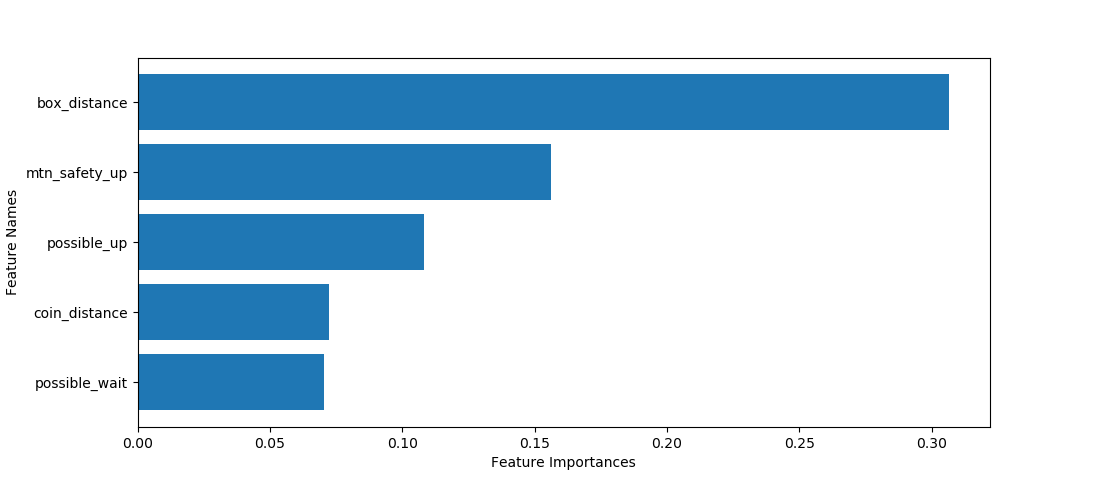
\includegraphics[width=\textwidth]{plots/UP_feature_importances.png}
\caption{UP Regression Tree Feature Importances top 5}
\label{up_feature_importances}
\end{figure}


\begin{figure}[h]
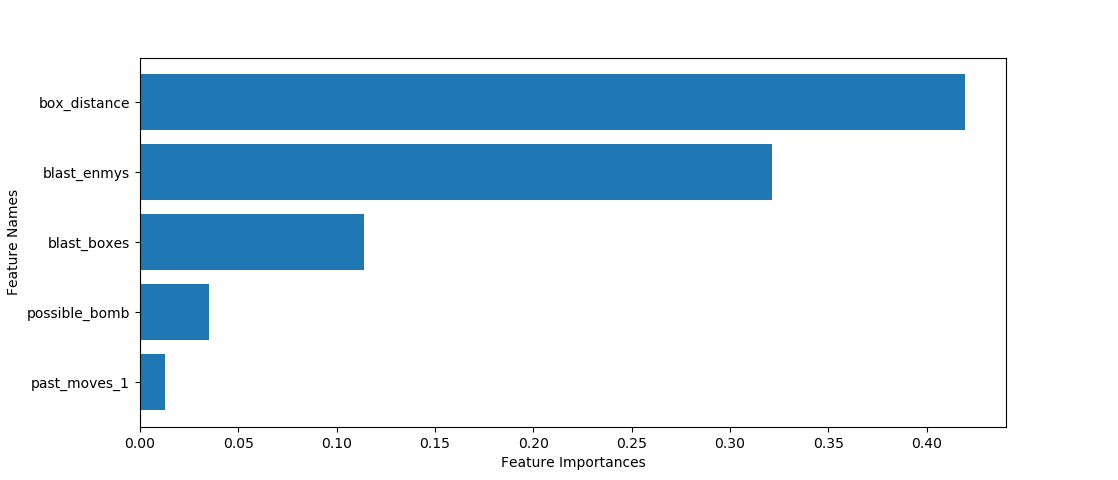
\includegraphics[width=\textwidth]{plots/BOMB_feature_importances.png}
\caption{Bomb Regression Tree Feature Importances top 5}
\label{bomb_feature_importances}
\end{figure}

Using decision trees instead of random forests to fit the training data gives more insight into how the features are utilized for prediction. Figure \ref{up_decision_tree} and figure \ref{bomb_decision_tree} show the decision trees for the “UP” and “BOMB” actions. It has to be noticed, that for simplicity, the fitted tree has a very low max\_depth and that its game performance is not comparable to the random forest. As seen in figure \ref{up_decision_tree}, the tree predicts the highest values for the “UP” move if there exists a path to a box (box\_distance $>$ -1) and the “UP” action, moves the agent in the direction of safety (mtn\_safety\_up $>$ 0). Figure \ref{bomb_decision_tree} shows, that the tree predicts the highest values for the “BOMB” action if there exists a path to a box (box\_distance $>$ -1), there is at least one enemy in blast range (blast\_enmy $\geq$ 1) and there is at least one box in blast range (blast\_boxes $\geq$ 1).

\begin{figure}[h]
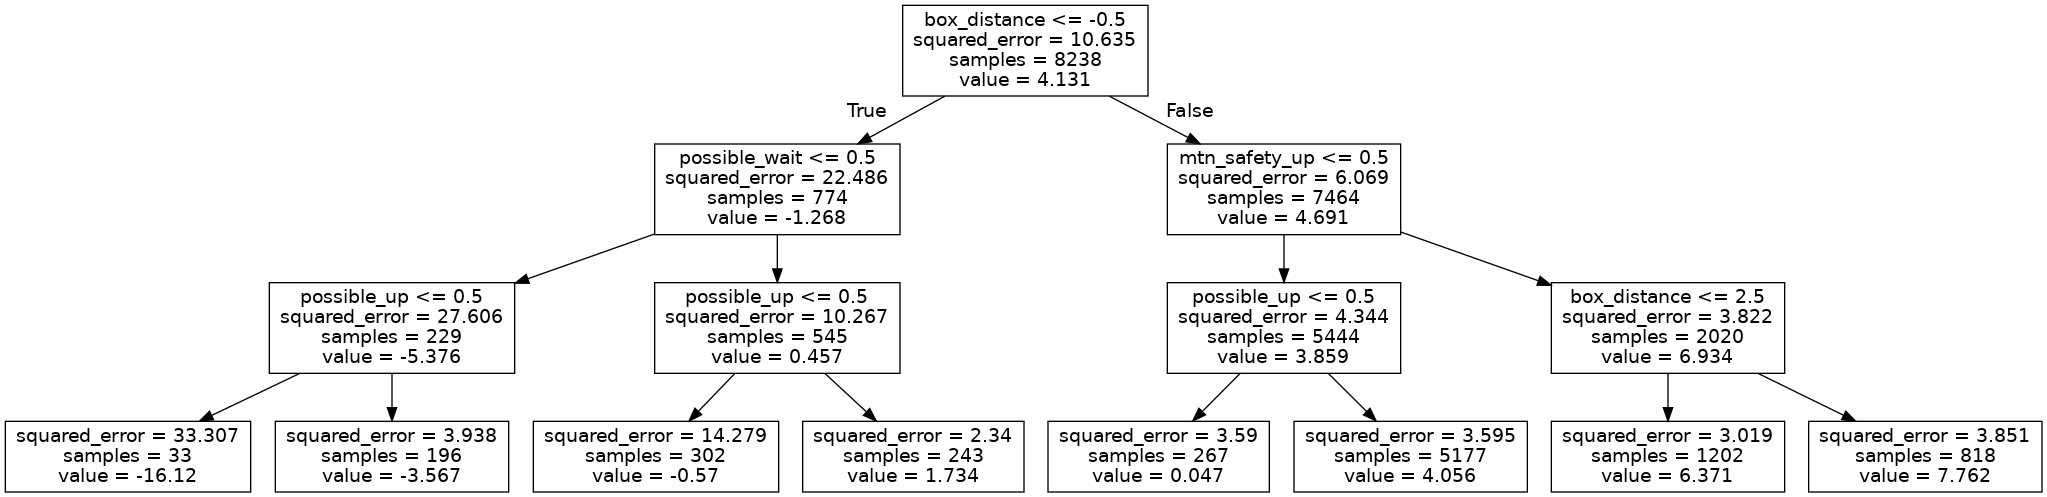
\includegraphics[width=\textwidth]{plots/UP_tree.png}
\caption{UP Decision Tree Regressor}
\label{up_decision_tree}
\end{figure}


\begin{figure}[h]
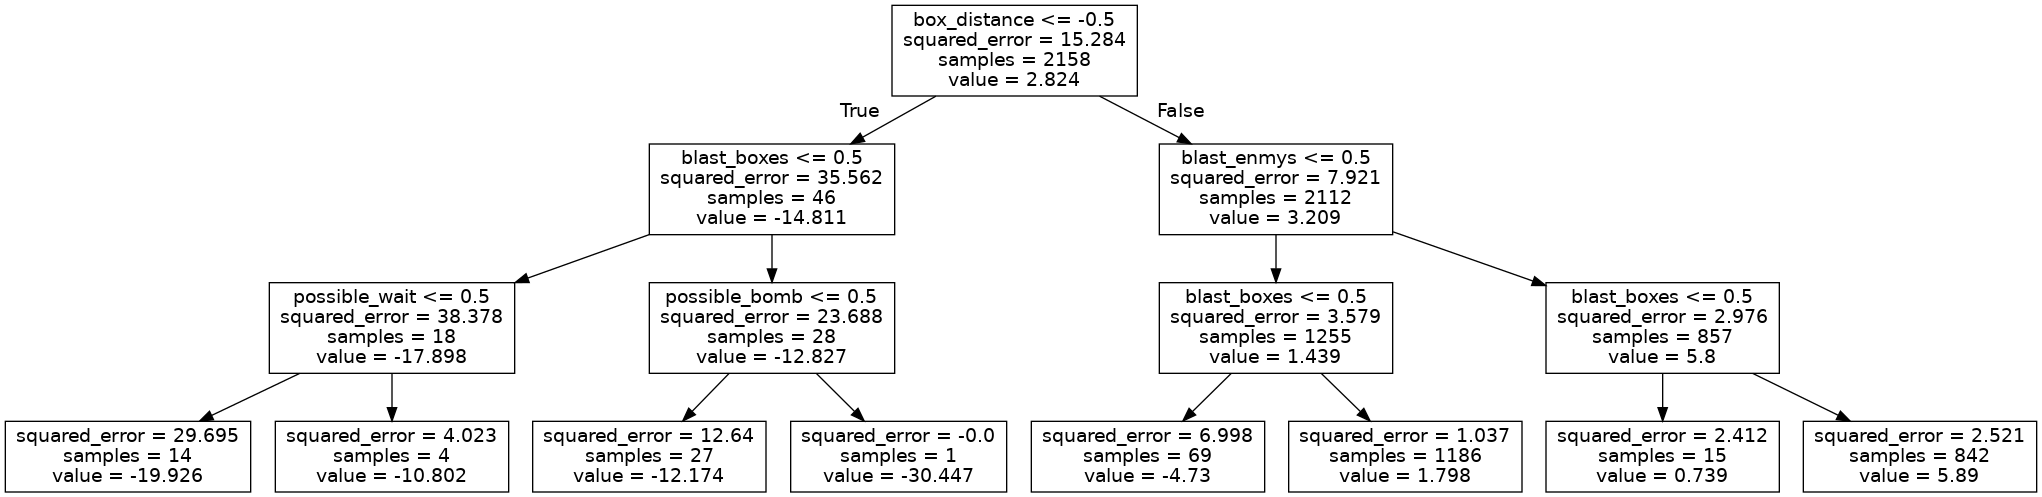
\includegraphics[width=\textwidth]{plots/BOMB_tree.png}
\caption{Bomb Decision Tree Regressor}
\label{bomb_decision_tree}
\end{figure}


Additional features we wanted to add but either did not have time to implement or which at first glance delivered poor results were:

\begin{enumerate}
    \item steps: The current step of a round could be used by the agent to “change its strategy” throughout the game, by for example changing the importance of actions.
    \item boxes: The number of boxes in the game could also be used by the agent to change its strategy, as it is less likely to corner and eliminate enemies with few boxes left.
    \item available\_coins: As each game has only a fixed amount of coins, providing the agent with the number of coins left to collect could prevent the agent from destroying boxes unnecessarily.
    \item enemy\_scores and own\_score: Values indicating the score of the agent and each enemy could be used to recognize when it is the best move for the agent to eliminate itself if it is unlikely to eliminate an enemy, and it cannot collect any further coins
\end{enumerate}

\subsection[Feature Engineering]{Feature Engineering {\small - Samuel Melm}}

A model can only be as good as the data it is fed, and preprocessing this data can go a long way. We soon noticed that bugs in the feature extraction code were hard to debug, and the code become hard to follow very quickly. To alleviate this, we resorted to basic methods of software engineering. We defined a base class for features with \ref{code:feature_class}.

\begin{figure}
\centering
\begin{minted}[frame=lines,
framesep=2mm,
baselinestretch=1.2,
fontsize=\footnotesize,
linenos]{python}
class Feature(metaclass=ABCMeta):
    def name(self):
        return camel_to_snake_case(type(self).__name__)

    @abstractmethod
    def dim(self) -> int:
        pass

    @abstractmethod
    def compute_feature(self, game_state: dict, self_obj) -> np.array:
        pass

    def format_feature(self, feature_vector: np.array) -> str:
        return str(feature_vector)

    def explain_feature(self, feature_vector: np.array) -> str:
        return f"{self.description()}: {self.format_feature(feature_vector)}"
\end{minted}
\caption{Feature class}
\label{code:feature_class}
\end{figure}

For every feature we wanted to extract from the game state, we created a new subclass. For common feature types, we defined subclasses to avoid code duplication and adhere to the DRY principle. These include two-dimensional features, boolean and action features. Each would implement a way to compute a vector from the game state and to format the resulting vector in a human-readable format. It would also provide the length of the vector it is computing. This allowed us to create a FeatureCollector class that also implements the feature interface. This class takes multiple features and combines them. It collects all computed vectors and concatenates them into one large feature vector. It also defines a custom explain\_feature function that creates a human-readable summary of the entire feature vector by delegating its parts to the sub-features using the dimension information. Such a summary can be seen in figure \ref{feature_summary}.

\begin{figure}[h]
\centering
\begin{verbatim}
    
****** feature summary *******

move to nearest coin: NONE
move out of blast zone: NONE
move next to nearest box: DOWN
agent in blast zone: no
possible actions: [1. 1. 1. 0. 1. 1.]
boxes in blast range: [0.]
could escape own bomb: yes
move to nearest enemy: RIGHT
past moves: [3. 3. 3. 3.]
enemies in blast range: [0.]
agent field neighbors: [ 0.  0.  0.  0.  0. -2.  0.  0.]
agent explosion neighbors: [ 0.  0.  0.  0.  0. -1.  0.  0.]
nearest enemy possible moves: [-1.]
safety distance: [-1.]
enemy distance: [8.]
box distance: [2.]
coin distance: [-1.]

*** end of feature summary ***
\end{verbatim}
\caption{Automatically generated feature summary}
\label{feature_summary}
\end{figure}

This makes debugging and creation of new features a lot easier. It also makes it a lot easier to organize the code.

\subsection[Learning]{Learning {\small - Jonas Gann}}

To learn the state-action rewards, we used q-learning, utilizing random forests for predicting future rewards.

\begin{figure}[h]
\centering
\begin{minted}[frame=lines,
framesep=2mm,
baselinestretch=1.2,
fontsize=\footnotesize,
linenos]{python}
self.action_value_data = {"UP": {}, "DOWN": {}, "LEFT": {}, "RIGHT": {}, "WAIT": {}, "BOMB": {}}
\end{minted}
\caption{Action Values}
\label{code:action_values}
\end{figure}

The experiences of games are stored as key value pairs, where the old game state is the key and the reward is the value. To distinguish the actions which achieved the reward, the state-reward pairs are inserted in the object corresponding to the performed action, as shown in figure \ref{code:action_values}.

\begin{figure}[h]
\centering
\begin{minted}[frame=lines,
framesep=2mm,
baselinestretch=1.2,
fontsize=\footnotesize,
linenos]{python}
score_diff = new_game_state["self"][1] - old_game_state["self"][1]

old_features = self.feature_collector.compute_feature(old_game_state, self)
new_features = self.feature_collector.compute_feature(new_game_state, self)

rewards = _rewards_from_events(self, old_features, events, self_action, score_diff)

q_value_old = self.trees[self_action].predict(old_features.reshape(1, -1))
q_value_new = rewards + DISCOUNT * np.max(
    [self.trees[action_tree].predict(new_features.reshape(1, -1)) for action_tree in self.trees]
)
q_value_update = LEARNING_RATE * (q_value_new - q_value_old)
self.action_value_data[self_action][tuple(old_features)] = q_value_old + q_value_update
\end{minted}
\caption{Q-Learning}
\label{code:temporal_difference}
\end{figure}

As shown in figure \ref{code:temporal_difference} the learning algorithm proceeds as follows: It first computes features from the old and new game state. The algorithm then goes on to compute the rewards based on the old game state and the events using a specifically crafted reward function.
It then computes the prediction of the reward for the state-action pair using the current model. This is done, as especially in the beginning for most game states there does not exist any experience, however, using the regression model, a reward can be predicted based on experience of similar game states. To improve the algorithm, it may be possible to check if the identical game state has already been experienced along with the action. In that case, the stored value could be used instead of a prediction. To compute the actual rewards, the algorithm adds the discounted reward of the best expected move for the new game state to the observed reward. Using the learning rate, the algorithm then updates the value of the experience stored in the action value object. This was our initial approach and delivered good results. We therefore did not invest much time in exploring different solutions. We took a quick look at n step temporal difference learning, but as there seemed to be a programming error somewhere, we returned to the solution described above. For more details about the performance of the training algorithm, see section \ref{section:experiemnts}.

\subsection[Predicting]{Predicting {\small - Jonas Gann}}

We early on focused on decision trees for prediction of rewards. The reason was that decision trees are very powerful in predicting non-linear features as well as having the option to take a look at the graph based visualization of the conditions. Their method of predicting also fits the given problem very well: Decision trees find thresholds for features which best separate the given data. We chose to use many one-hot and boolean features. Decision trees can “find” the values of the one-hot encoding which are relevant (selecting features which best reduce the impurity). 
The “UP” tree for example might select the first value of the one hot encoding, which indicates if the “UP” move leads to the point of interest. 
The model can then predict a value based on the fact that features are on or off. As a result of that, even though one-hot encoding results in a large feature vector, each decision tree only uses the features which are relevant for it.
The “BOMB” tree on the other hand might select the numerical value indicating how many boxes are in range.

We also tried to craft feature vectors for each decision tree individually. Each decision tree would then get a feature vector indicating whether its action would for example move the agent towards a coin or would destroy a box. However, we noticed, that it can be important for each of the trees to not only know if for example their action moves the agent to a coin but also know whether any of the other action would move the agent towards a box. We therefore decided to accept the negative effect of the large feature size and used one-hot-encoding to create identical features for the trees. We chose not to encode the features using numerical values to avoid the model assuming that the actions are ordered.

We initially used decision trees because of their ability to easily output the resulting tree structure. Later on we exchanged them by random forests to take advantage of their better behavior regarding overfitting. We decided to use 6 random forest regressors, one for each possible action. Each forest predicts the expected reward for a game state if the action of the forest were to be performed. With this method we achieved good results compared to other regression methods. For more details, see section \ref{section:experiemnts}.

\begin{figure}
\centering
\begin{minted}[frame=lines,
framesep=2mm,
baselinestretch=1.2,
fontsize=\footnotesize,
linenos]{python}
new_trees = {}
for action in Actions:
    action = action.name
    action_value_data_action = action_value_data[action]
    features = []
    values = []
    for key in action_value_data_action:
        feature = np.array(key)
        value = action_value_data_action[key]
        features.append(feature)
        values.append(value)
    new_tree = RandomForestRegressor()
    features = np.array(features)
    values = np.ravel(np.array(values))
    X_train, X_test, y_train, y_test = train_test_split(features, values, test_size=0.33)
    new_tree.fit(X_train, y_train)
    new_trees[action] = new_tree
return new_trees
\end{minted}
\caption{Fitting Random Forests}
\label{code:random_forest}
\end{figure}

To train the forests accordingly, the algorithm performs the following computations for each action: Initially, all experienced rewards after performing the action are retrieved. This means, the forest is only fitted using rewards which resulted from performing “its” action. Then a new forest is created and fitted using the game states and rewards stored in the experience. The newly trained tree is then stored as the new model. As described, in this implementation, all experience of all played games is used to train the forests. It would be interesting to see the effect of using an experience buffer which only uses the last n entries for training, therefore forgetting very old values and speeding up training. Due to time constraints, we did not test this option.

\subsection[Training]{Training {\small - Jonas Gann, Samuel Melm}} \label{sec:training}
% Training. Describe your training process, including all tricks employed to speed it up (e.g. self play strategy, design of auxilliary rewards, prioritization of experience replay and so on).

Our model has a few hyperparameters which are relevant for training.

\begin{itemize}
    \item discount rate $\gamma$: How much the agent should look into the future. The lower this value is, the less rewards some steps ahead matter.
    \item exploration rate $\epsilon$: How often should the agent just randomly try something new? This helps to prevent that the agent gets stuck in a local minimum.
    \item $\epsilon$-decay rate: Said chance of trying something different gets smaller by this factor the more the agent learns. Otherwise, the upper bound for the performance is limited by the random moves the agent does for exploration.
    \item $\epsilon$-minimum: The smallest value the exploration rate is limited to take.
    \item learning rate $\alpha$: How much the agent should change its predictions depending on how wrong the current one was.
\end{itemize}

For training the agent, we started with a learning rate of 0.1, a discount of 0.95, an epsilon of 1, a minimal epsilon of 0.01 and an epsilon decrease rate of 0.95. These values seemed to give a good starting point for a model. Once a decent model was found, we reduced the learning rate to 0.01 and epsilon to 0.01 for further optimization. As we noticed, that training of the models for a large amount of time (overnight) would eventually decrease the game performance of the agent, we stored each trained model in a separate file along with the average score it achieved. This enabled us to eventually select the best performing model. The model was trained after every fifth round.

Initially we started to reward the agent by simply assigning fixed rewards for each of the predefined events (coin collected, died, enemy killed, box destroyed, …). As this turned out to be insufficient, we successively added more rewards based on the features we computed.

\begin{figure}[h]
\centering
\begin{minted}[frame=lines,
framesep=2mm,
baselinestretch=1.2,
fontsize=\footnotesize,
linenos]{python}
if action_to_safety != Actions.NONE:
    if action == action_to_safety: rewards += 1
    else: rewards -= 1
elif action_to_coin != Actions.NONE:
    if action == action_to_coin: rewards += 1
    else: rewards -= 1
elif can_place_bomb and bomb_good and (blast_boxes > 0 or blast_enemies > 0):
    if action == Actions.BOMB: rewards += 1
    else: rewards -= 1
elif action_to_box != Actions.NONE:
    if action == action_to_box: rewards += 1
    else: rewards -= 1
elif action_to_enemy != Actions.NONE:
    if action == action_to_coin: rewards += 1
    else: rewards -= 1
\end{minted}
\caption{Reward Shaping (Rule Based)}
\label{code:reward_shaping_1}
\end{figure}

Our first approach to adding more detailed rewards resulted in the rewards shown in figure \ref{code:reward_shaping_1}. Using elif statements, we “hard-coded” a priority of actions: Foremost if the agent has to escape, he should do that (positive reward) otherwise he is punished (negative reward). If the agent does not have to escape, he should collect a coin if there is one, and so on. This resulted in pretty good performance. However, as we continued to think about it, we asked ourselves what the fundamental difference to a conventional rule based agent exists: The model is trained to exactly mimic the if/else rules we specified through rewards. Therefore, the agent was not able to find strategies of its own, defeating the whole purpose of machine learning. Therefore, we continued to give the agent more freedom in learning.

\begin{figure}[H]
\centering
\begin{minted}[frame=lines,
framesep=2mm,
baselinestretch=1.2,
fontsize=\footnotesize,
linenos]{python}
local_rewards = 0
global_rewards = 0

if action_to_safety != Actions.NONE:
    if action == action_to_safety: local_rewards += 7
if action_to_coin != Actions.NONE:
    if action == action_to_coin: local_rewards += 3
if can_place_bomb and bomb_good and (blast_boxes > 0 or blast_enemies > 0):
    if action == Actions.BOMB: local_rewards += 1
    if action != Actions.BOMB and action_to_safety == Actions.NONE: local_rewards -= 1
if can_place_bomb and bomb_good and not (blast_boxes > 0 or blast_enemies > 0):
    if action == Actions.BOMB: local_rewards -= 8
if action_to_box != Actions.NONE:
    if action == action_to_box: local_rewards += 1
if action_to_enemy != Actions.NONE:
    if action == action_to_enemy: local_rewards += 1

if e.COIN_COLLECTED in events: global_rewards += 40
if e.CRATE_DESTROYED in events: global_rewards += 10
if e.KILLED_OPPONENT in events: global_rewards += 100
if e.GOT_KILLED in events: global_rewards -= 100
if e.WAITED in events: global_rewards -= 0.5

if action_to_box != Actions.NONE and action_to_enemy == Actions.NONE and action_to_coin == Actions.NONE:
    if action == action_to_box: global_rewards += 10
if action_to_coin != Actions.NONE and coin_distance < 5:
    if action == action_to_coin: global_rewards += 10
if nearest_enemy_possible_moves <= 1 and enemy_distance <= 3 can_place_bomb and bomb_good and blast_enemies > 0:
    if action == Actions.BOMB: local_rewards += 10
rewards = local_rewards + global_rewards

return rewards
\end{minted}
\caption{Reward Shaping (Learning)}
\label{code:reward_shaping_2}
\end{figure}

The rewards shown in figure \ref{code:reward_shaping_2} are the ones we eventually used for the submitted agent. Here, we defined two types of rewards: “local” rewards and “global” rewards. The purpose of the small local rewards is to give the agent early feedback to push him roughly in the right direction to a global optima, however, the local rewards limit the freedom of the agent and lead to a bad local optimum. For example, the agent could gain infinite rewards by moving back and forth towards a nearest coin and a nearest box. For the agent to eventually reach a good global optimum, we added large global rewards which have direct influence on the game score. These are e.g., the coins collected, the crates destroyed, etc. As these rewards do not occur as often as the local rewards and as they should be able to “overwrite” bad local optima, we scaled the global rewards with a factor between 10 and 100. The local rewards in figure \ref{code:reward_shaping_2} look similar to the rewards shown in figure \ref{code:reward_shaping_1}. However, in figure \ref{code:reward_shaping_2}, there exist no else statement. Instead, the importance of actions is indicated by their specified reward. This gives the agent more freedom to learn. One example is, that the agent in this case prefers to walk in the direction of multiple points of interest. As we noticed some unwanted behavior of the agent if there existed no enemies, where the agent would stand still and not collect coins or destroy boxes, we added some explicit rewards to collect coins and destroy boxes when no enemies exist. The last reward, in line 33, proved to be a useful incentive to the agent to place bombs next to enemies which have at most one possible way to move. This is supposed to corner enemies with bombs and eliminate them. To our surprise, this worked pretty good, and the agent would approach enemies with few movement options and place a bomb.


\subsection[Experiments and Results]{Experiments and Results {\small - Samuel Melm}}
\label{section:experiemnts}

To validate our graph algorithm and feature engineering, we wanted to prove the hypothesis that the MoveToNearestCoin feature is enough to reach a good performance in the coin heaven scenario. For this, we ran the scenario without opponents and trained our agent with $\epsilon=0.95$ and $\alpha=0.3$. The results can be seen in figure \ref{fig:coin_heaven_only_nearest_coin} and indicate that this single feature is indeed enough for our agent to learn to perform reasonably well in the coin heaven scenario.


\begin{figure}[h]
    \centering
    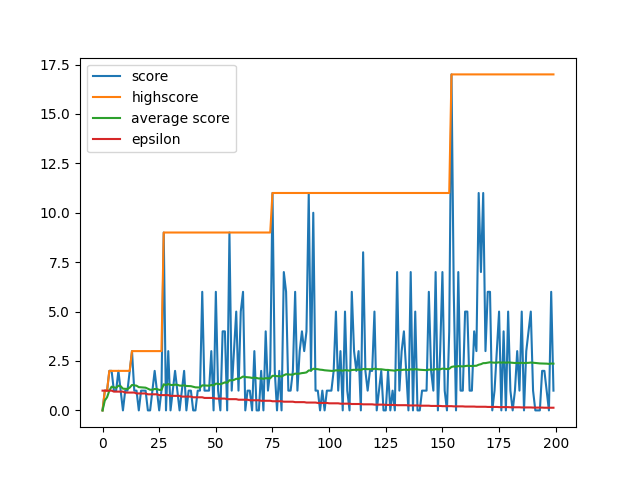
\includegraphics[scale=0.6]{plots/coin_heaven.png}
    \caption{Scores in coin-heaven with only the MoveToNearestCoin feature as the feature vector}
    \label{fig:coin_heaven_only_nearest_coin}
\end{figure}

To verify that our training works properly, we trained our agent against three rule-based agents for 200 rounds. Every fifth round we trained our agent and recorded the results, which can be seen in figure \ref{fig:scores}. This shows that our agent can learn rather fast, and more notably that its peak performance seems to happen at the 150 round mark.

\begin{figure} [h]
    \centering
    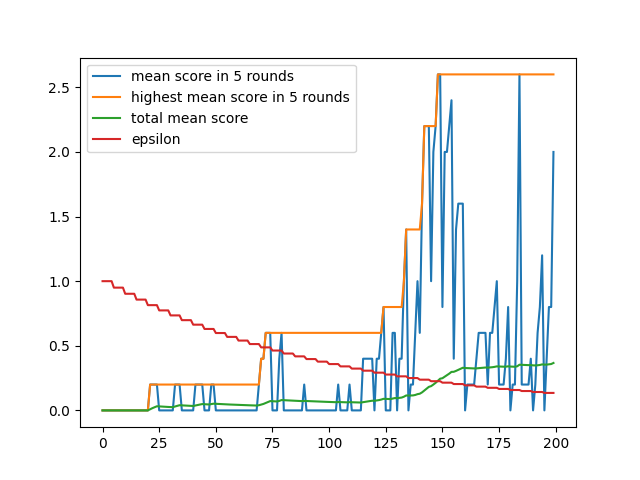
\includegraphics[scale=0.6]{plots/scores.png}
    \caption{Scores during training against three rule-based agents}
    \label{fig:scores}
\end{figure}

We decided early on that we wanted to use trees or forests as our regression model, with linear regression as a second choice. We spent a lot of time optimizing our tree-based model and to verify that our decision we ran a comparison experiment between the different regression methods. We compared linear, ridge, support vector, decision tree and random forest regression. Additionally, we tested three different neural networks with a single hidden layer of size 20, 40, and 60 respectively. 

The results can be seen in figure \ref{fig:scores_and_steps}. The first plot shows the average between the training and test score for each action. Note that this starts at round thirty because some methods tend to have a large negative score in the early rounds, which causes problems in the scale of the plots. The second plot shows the step count per turn and the current highest achieved step count, which can be used as an approximation for agent performance. Unfortunately, due to a problem in the script that collected this data, we are unable to show the actual scores. These plots show that tree-based methods and ridge regression outperform the alternatives, affirming us in our choice of regression method. You may notice that linear regression is missing from the plots. When creating the plots, we noticed that linear regression tended to create large spikes in the graph. We assume this is caused by overfitting, which with bad luck during the splitting into test and train dataset causes large errors. Since these render all other graphs unreadable and can occur at any step, we decided to drop linear regression, which seemed to perform worse than ridge regression anyway.

\begin{figure}[h]
    \centering
    \begin{minipage}[c]{\textwidth}
    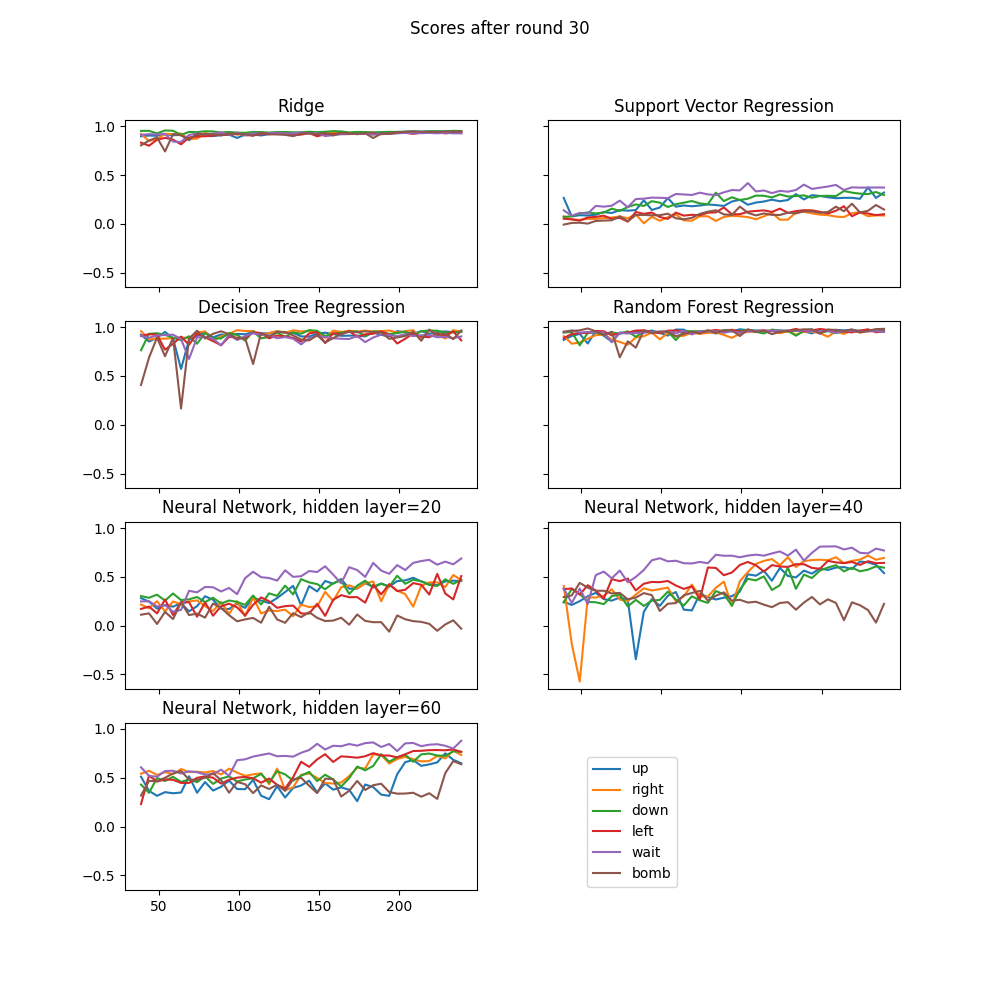
\includegraphics[scale=0.3]{plots/model_scores_after_round_30.png}
    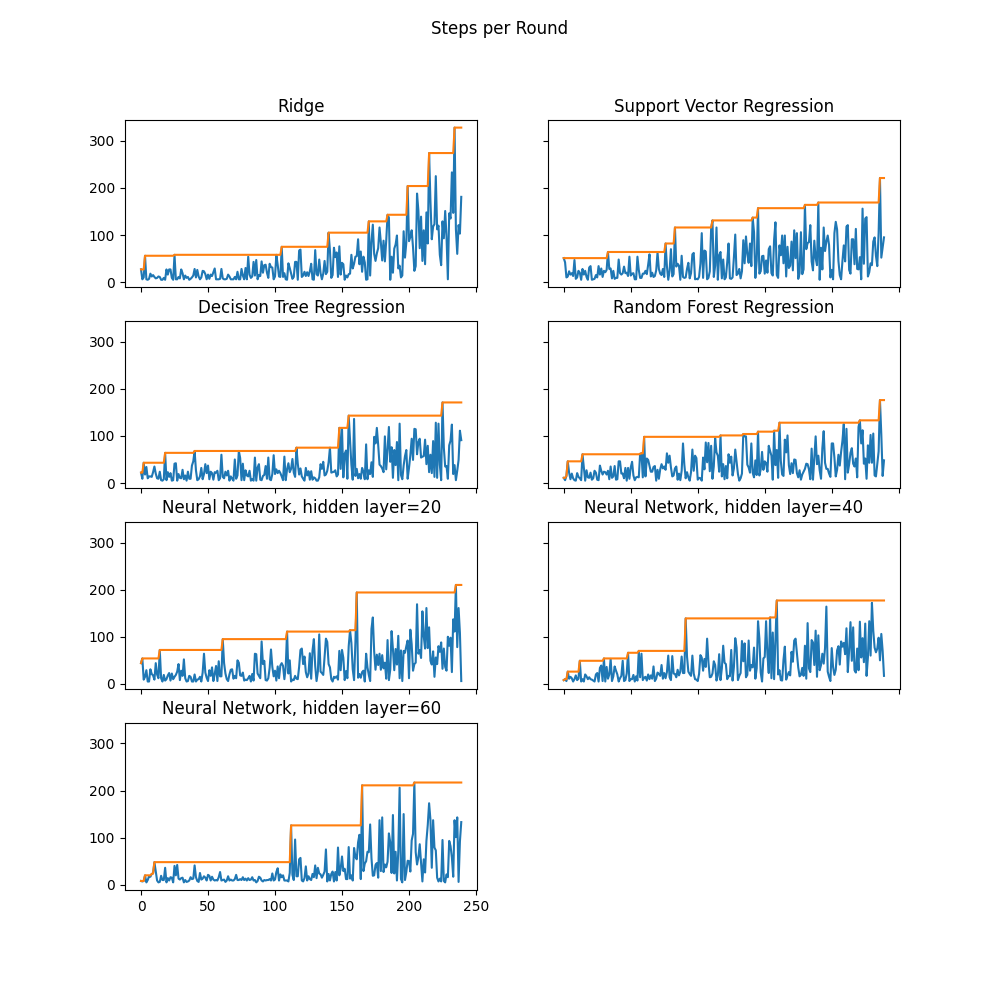
\includegraphics[scale=0.3]{plots/steps_per_round.png}
\end{minipage}

    \caption{Scores and steps per round for different regression methods.}
    \label{fig:scores_and_steps}
\end{figure}


\section[Neural Network Agent]{Neural Network Agent {\small - Samuel Melm}} \label{sec:nn_agent}

For our second agent, we wanted to take a different approach. We wanted to see what could be achieved by simply relying on a huge amount of data. Our plan was to record a lot of games of the rule-based agent and derive the returns for each step. Since the rule-based agent already achieves an impressive performance, we figured that if our agent would simply replicate its behavior, it would be a good jumping off point. The obvious problem with this approach is that the rule-based agent simply does not do some errors you would want your agent to learn to avoid first (e.g., killing itself with its own bomb). To get around this we decided to include the other agents (random, peaceful, coin-collector) which should provide a sufficiently diverse set of performed actions. 

We wrote a script that iterated over each combination of the four agent types and saved the game state for each of them into a pandas data frame. Each combination formed a batch, but since we had to restart the process several times to tweak the number of rounds per batch it resulted in 55 batches being collect, each consisting of 50 to 100 rounds each. The resulting dataset had, 980430 rows which correspond to one game step. But since each row contains information about four agents, the actual size of the dataset was therefore nearly four million.

Mostly out of curiosity, we applied principal component analysis to the dataset to visualize it, which resulted in figure \ref{fig:data_pca}. The distribution in the center was expected, but we found the rectangular shape surprising. We suspect that the large number of one-hot encoded vectors and the fact that most of the data lies in small intervals to be responsible for it. More interesting are the corners of the rectangle, which show a much higher density. Our guess is that this represents the starting positions. 

\begin{figure}[h]
    \centering
    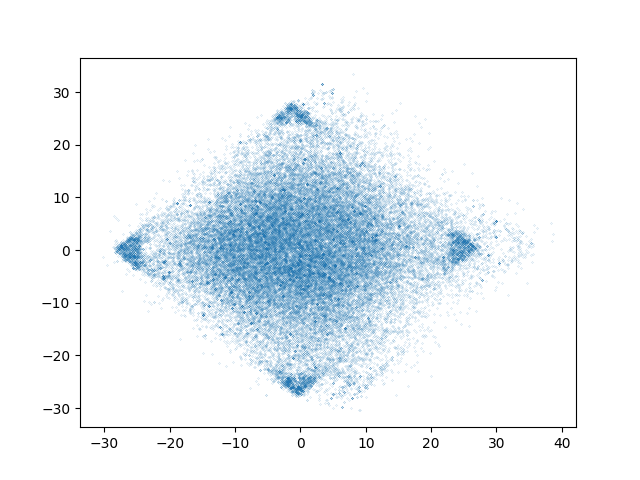
\includegraphics[scale=0.6]{plots/big_data_pca.png}
    \caption{PCA of the collect data. For visual clarity, only half the dataset was randomly sampled.}
    \label{fig:data_pca}
\end{figure}

Since all the games were already played out, we did not have to resort to temporal difference learning and only use the next step to predict the reward, but could directly compute the actual returns for each step starting from the last. Since it was rather cumbersome to collect both the game states and the computed rewards, we only collected the former. This meant that while we could more accurately pinpoint the effect each step had on the resulting reward, we were limited in our reward shaping. We decided to just use compute the discounted returns from the awarded score.  

In the next step, we needed to compute the feature vectors for each entry, where we quickly discovered the downside of such a large dataset. Since our graph algorithm cannot be vectorized, the feature vectors need to be computed sequentially. Since the graph algorithm is written in pure Python, it is significantly slower than any other NumPy operation would be. Before we started the computation, we timed a small sample and did some paper napkin math through which we discovered that it would take nearly a day to compute the feature vectors for one of the four agents which is just 25\% of the entire dataset. This was not acceptable, of course. We noticed rather quickly that the main problem was that there is no default implementation for a parallel apply in pandas, which means that even one a reasonably fast multicore machine, there is no speedup to be expected. We started to look into ways of parallelizing the process. We tried \href{https://github.com/modin-project/modin}{modin} as well as the underlying \href{https://docs.dask.org/en/stable/}{dask}. Both seem to be terrific libraries, judging by the documentation and the recommendations on Stack Overflow. Interestingly, we quickly discovered that the computation was even slower than using a vanilla Python loop. We suspect that the overhead that allows these libraries to run pandas operation on entire computer clusters has too large of an impact in the context of our rather humble goal of running on eight cores.

When dask based approaches did not seem to work, we tried the library \href{https://github.com/nalepae/pandarallel}{pandarallel} which worked like a charm. We set it up to use seven of eight cores in order to be still able to use the device in the meantime. With these settings, it continuously was able to use between 95 to 100\% of the available CPU power, which resulted in a six-fold speedup. It took six hours for pandarallel to compute the feature vectors for the first agent. Sadly, it crashed once all processes were done. At least we think it crashed, since the process did not finish, even three hours after all workers were done. We suspect that there was a problem collecting and concatenating the processed data, but that is only speculation. We started it again, this time partitioning the data in smaller chunks, but it seemed like something broke in the library which raised an internal error every time we started it. Neither clearing the cache nor reinstalling it could fix the problem.

At this point, we gave up on the smart approaches to the problem and just let a simple for loop run overnight. This processed the data of one and a half agents, and over the next day we repeated it for another half of an agent. At this point we accepted that this was enough data and that we probably overdid it.

Once we had a finished dataset, we applied different regression methods to it, to find out which would work best. We most relevantly tried linear and ridge regression and neural networks. We quickly realized that a neural network with a single hidden layer with a size somewhere between 20 and 60 outperformed the other methods by far, but even then its performance was bad. Not a single model achieved a test score above $0.1$\footnote{the scores for data from the training set interestingly were even worse, mostly negative. A fact we still cannot explain.}. The plan was to use this data as a sort of pretraining that could be refined during self-play but in the light of these results and the comparison \ref{fig:scores_and_steps} where neural networks did not perform as well as the other methods, we decided that this approach was a dead end and not worth spending more time on. We therefor scratched this approach completely\footnote{the code for it can still be found in the \href{https://github.com/J-Gann/FML/tree/main/bomberman_rl/agent_code/fail_agent_nn}{repository} } and present a version of our first which uses ridge regression instead of a random forest as our \href{https://github.com/J-Gann/FML/tree/main/bomberman_rl/agent_code/null_agent_rigde}{second model}. This model performs nearly as well as the one using a forest. While the outcome of this second approach is quite unfortunate, the time spent on it was not entirely wasted since some valuable lessons could be learned from its failure, which we will present in our conclusion in section \ref{sec:conclusion}.


\section[Conclusion]{Conclusion {\small - Samuel Melm}} \label{sec:conclusion}

We learned a lot during this project, both from our successes and from our failures. In this chapter, we will discuss these experiences and how they would change our approach, were we to do this project again.

\subsection[Lessons Learned from Failure]{Lessons Learned from Failure {\small - Samuel Melm}}

While the approach outlined in section \ref{sec:nn_agent} was not as successful as we hoped it would be, it still taught us some valuable lessons. While we had prior experience with the pandas framework, neither of us had ever worked with a dataset of such proportions. We realized that there are different strategies that need to be applied when working with that amount of data:

You need to act more carefully: When your current state of the data took half an hour to compute, you do not want to risk losing deleting it by making a typo.  

Checkpoints can be a lifesaver: This is a corollary of the previous point. When you make an effort to save every intermediate step that was expensive to compute, you do not run into the risk of losing a lot of time due to errors. Even more importantly, this also protects from data loss when a long-running computation crashes. Partitioning the data and saving the results more frequently may be slower, but it assures that not all progress can be lost at once.


You need to plan ahead and manage your resources: There is an instinct in any project to not waste time on anything that does not directly result in progress. We discovered that this instinct is misplaced once the ratio of work the human and the computer does shifts. When most of the work time is spent waiting for numbers to be crunched or models to be fitted, it is a lot more important to plan ahead and reduce that time. It proved as vital in this task to calculate beforehand how long a computation will likely run and to prepare it in a way it uses the given resources as optimally as possible.

Feedback and sanity checks are important: Every CPU cycle wasted inside a for loop that runs a million times feels bad. We made the experience that computation time that informs about the status is worth it. When working in an interactive environment, it is important to know whether it is worth waiting for a computation to finish. Tools like tqdm and its integration with pandas are crucial for this.

Data is not everything: In our second approach, we fell victim to the “big data” mindset. We thought that the more data we threw at the problem, the better the result would turn out to be. We underestimated the challenges that the quantity of data would bring and while trying to overcome them lost sight of the quality of the data. It was surprising to us how little use the pretraining with the collected returns had, but it seems to prove \href{https://en.wikipedia.org/wiki/Garbage_in,_garbage_out}{garbage in, garbage out} principle. In the future, we will keep in mind that you should only use as much data as you can assure the quality of.

\subsection[Lessons Learned from Success]{Lessons Learned from Success {\small - Samuel Melm}}

While our second approach (section \ref{sec:nn_agent}) performed below our expectations, our first approach outlined in section  \ref{sec:submitted_agent} performed above them. It learns to play the game well in a reasonable amount of time.

The main lesson we learn from this is the importance of good feature engineering and reward shaping. At the beginning, we spend a lot of time on this, but it set up the success of the entire project.

One thing that will become apparent in section \ref{sec:what_to_improve} is that we wished that we spent more time learning about and exploring other possibility, especially learning and regression methods, instead of fine-tuning a decent model further and further. If we kept this in mind from the beginning, we could have designed our system in such a way that allowed experimentation with and comparison of different models more easily. 

\subsection[Possible Further Improvements]{Possible Further Improvements {\small - Samuel Melm}} \label{sec:what_to_improve}

In this chapter, we discuss what we would do if we had more time to improve our agent.

\subsubsection[Automated Hyperparameter Tuning]{Automated Hyperparameter Tuning {\small - Samuel Melm}}

There are a few hyperparameters that modify the training and prediction behavior of our model. In addition to the parameters outlined in section \ref{sec:training} there is also the choice of regression method and the hyperparameters specific to that method. Finding the best values for these parameters is one of the core challenges in any machine learning project. Our approach consisted of simply trying different combinations and gaining an intuition for the impacts each parameter has on the results. There are two major problems with this approach. For one, it becomes hard to quantify and substantiate the developed gut feeling with actual data. To mitigate this (especially for long-running projects) a system to log the different experiments with their parameters and results would be needed. Tools like \href{https://github.com/IDSIA/sacred}{sacred} would work well for this. The bigger problem is that we can never be sure whether we missed that one set of parameters that would be perfect for the problem at hand. To reduce the uncertainty, we could employ a system that automatically searches the parameter space for the best combinations. Sklearn offers functionality to perform an \href{https://scikit-learn.org/stable/modules/grid_search.html}{exhaustive grid search}. Another option would be to perform some sort of genetic algorithm, which leads us to our next point.

\subsubsection[Heterogeneous Models and Genetic Algorithms]{Heterogeneous Models and Genetic Algorithms {\small - Samuel Melm}}

Given more time, we would generally focus more on the self-play aspect of training. Our submitted model was mostly trained against the rule-based agent, but we believe that its performance would further increase if we created a training regiment that pitted it more against copies of itself with other agents like the rule-based agent added to the mix to prevent the model from overfitting to only beat itself.  

This could be further expanded by pitting versions of our agents against one another that use different regression methods or hyperparameters to model Q. This would allow us to definitively determine the best model.

The fact that our model actually consists of seven models (one per action) would allow us to take this even further. We could experiment with models that are a mixture of multiple others. Such a model could have a linear regression model to approximate Q for the up action, but model the down action with a decision tree. The left and right actions could both be modeled with neural networks, but they could have different hidden layer sizes. We could train these agents using a genetic algorithm. We would start with a large population (maybe 100 agents) initialized with a diverse set of regressors and hyperparameters. In each epoch they would fight each other in a tournament like arrangement where their performance is recorded. After the epoch, the selection would eliminate agents with a likelihood proportional to their performance. The survivors would then produce offspring which would be a combination of each of their genes, which are the individual regression models for the actions. This process could be further refined by introducing random mutations, which could be implemented in various different ways. In theory this process should lead to stronger and stronger agents where only the best genes survive. This could lead to interesting observations like what regression model performs better on modeling the bomb placing behavior, which is a lot more difficult because of the sparsity of data.  

\subsection[How the game setup could be improved]{How the game setup could be improved {\small - Samuel Melm}}

Overall, we were really happy with the setup provided for this project. The different command line options and scenarios made it quite easy to work on the project.When we tried to call then main function from another Python file, we noticed that while it takes an arg parameter, it ignores it. Another thing we looked into implementing ourselves was some mechanism to pass command line arguments to the agent(s). This could allow teams to pass hyperparameters via the command line, instead of hard-coding them, and would make things a bit easier. The easiest way of implementing this would be to allow any additional parameter and passing the entire args object to the agent during setup. 
The use of self as a parameter name for the callbacks become confusing in the later stages of the project, especially once we introduced classes that required a reference to that object. To avoid the clash with the Python OOP convention, we recommend a more expressive name like storage.

\end{document}
